\section{极值、最值与平衡}
\subsection{导数符号比零点方程包含更多信息}
在区间内部，若 $f'>0$，函数随自变量增大而增大；若 $f'<0$，则减小。可导函数在内点取得局部极值时，必有 $f'=0$，但这个条件只是候选条件。例如 $x^3$ 在零点导数为零，却始终递增，因此零点不是极值点。

判断候选点应看两侧导数：由正变负是极大，由负变正是极小；若导数不变号，通常不是极值。二阶导数判据是这一规律的局部形式：若 $f'(x_0)=0$，且 $f''(x_0)>0$，则附近向上弯曲，$x_0$ 为极小；若 $f''(x_0)<0$ 则为极大。二阶导数为零时必须继续分析，不能直接下结论。

闭区间上的连续函数必有最大值、最小值。求全局最值时，应把内部驻点、内部不可导点与端点一起比较。端点未必满足 $f'=0$，例如 $f(x)=x$ 在 $[0,1]$ 上的最大值位于 $1$。开区间则可能只有上确界或下确界，而没有实际取得该值的位置；定义域是解题步骤的一部分。

导数判单调的依据是有限变化也能由某个中间位置的变化率控制。若 $f$ 在 $[a,b]$ 上连续、内部可导，中值定理给出 $f(b)-f(a)=f'(\xi)(b-a)$。所以整个区间内导数为正时，任意从左到右的有限变化都为正。仅知道某一点导数为零，没有提供两侧有限变化的符号，自然不足以判断极值。

实际建模时先确定允许区间，再寻找候选位置。例如绳长、折射角、液面高度有各自边界，数学驻点可能落在不可实现区域。对含绝对值或接触切换的关系，还要把表达式发生变化的位置列入比较。得到候选点后代回函数值，而不是比较导数值，才能回答题目所问的最大量或最小量。

\fig{fv:c3:stationary}{同为水平切线，导数是否变号决定极值性质}{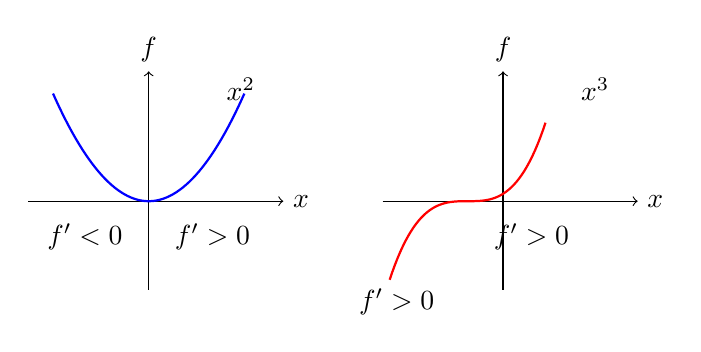
\begin{tikzpicture}[x=.9cm,y=.75cm]
\foreach \x/\lab in {0/{$x^2$},4.5/{$x^3$}}{\begin{scope}[xshift=\x cm]
\draw[->](-1.7,0)--(1.9,0)node[right]{$x$};\draw[->](0,-1.5)--(0,2.2)node[above]{$f$};\node at(1.3,1.9){\lab};\end{scope}}
\draw[blue,thick,domain=-1.35:1.35,samples=60]plot(\x,{\x*\x});
\draw[red,thick,domain=-1.1:1.1,samples=60]plot({4.5+\x},{\x*\x*\x});
\node at(-.9,-.6){$f'<0$};\node at(.9,-.6){$f'>0$};
\node at(3.5,-1.7){$f'>0$};\node at(5.4,-.6){$f'>0$};
\end{tikzpicture}}
图\ref{fv:c3:stationary}左图从原点左侧减小、右侧增大，原点确为极小点；右图经过原点仍递增，水平切线只表示瞬时斜率为零。因而解 $f'=0$是找候选点，读取两侧变化才完成判别。若自变量还限于闭区间，例如 $x^3$在 $[-1,1]$内求最值，最大、最小分别在端点，原点的驻点性质不能替代端点比较。


\subsection{势能导数与稳定性}
对一个广义坐标 $q$，保守力的虚功满足 $Q\,\dd q=-\dd U$，故 $Q=-U'(q)$。若 $q$ 是长度，$Q$ 为相应方向的力；若 $q$ 是角度，$Q$ 是力矩。不能不看坐标意义就把势能的一阶导数都称作同一种力。

平衡满足 $U'(q_0)=0$。作小位移 $\eta=q-q_0$，若
\[
 U(q)=U(q_0)+\tfrac12K\eta^2+\cdots,
\]
则恢复作用为 $Q=-K\eta+\cdots$。$K>0$ 时扰动受到恢复，称稳定平衡；$K<0$ 时扰动被放大，称不稳定平衡。若 $K=0$，应看更高阶：$+\eta^4$ 仍给出稳定平衡，$-\eta^4$ 不稳定，$\eta^3$ 也不能给出局部势阱。若一个区间内势能完全恒定，则在该坐标方向为随遇平衡。

稳定性还依赖允许的扰动。只准沿杆轴改变两球距离时的稳定，不等于对所有空间扰动都稳定。题设中的约束必须保留到判据中。

\fig{c3k-potential}{势能在平衡点两侧的变化决定扰动后的趋势}{\begin{tikzpicture}[x=1cm,y=.9cm]
\draw[axis](-2.2,0)--(2.5,0)node[right]{$q-q_0$};
\draw[axis](0,-1.9)--(0,2.1)node[above]{$U-U_0$};
\draw[world,blue,domain=-1.5:1.5,samples=40]plot(\x,{.65*\x*\x});
\draw[world,red,domain=-1.5:1.5,samples=40]plot(\x,{-.65*\x*\x});
\node[right,blue]at(1.55,1.46){$K>0$};
\node[right,red]at(1.55,-1.46){$K<0$};
\node[below left]at(0,0){$O$};
\end{tikzpicture}}
图 \ref{c3k-potential} 的蓝色曲线在平衡点两侧上升，向任一侧偏移都要增加势能，负梯度就把物体推回；红色曲线则相反。这里判定的是静态平衡位置对微小扰动的响应，不是说稳定系统一定最终停在平衡点。没有耗散时，稳定平衡附近通常发生往复运动；存在耗散时，才可能逐渐回到平衡点。

当二阶系数为零，继续求导只是找最低非零项的手段。若 $U-U_0=a\eta^{2n}$、$a>0$，两侧势能仍上升，因而仍稳定；若最低非零项为奇次幂，一侧势能下降，便不是局部势阱。对只允许单侧扰动的边界平衡，不能照搬双侧判据，应在真正允许的方向上检查势能变化。


图\ref{c3deep:quartic}把二阶判据失效时的三种情况画在同一尺度下。三条曲线在原点都满足一阶、二阶导数为零，但蓝线 $+\eta^4$ 在两侧都上升，红线 $-\eta^4$ 在两侧都下降，虚线 $\eta^3$ 则一侧升、一侧降。对蓝线，力 $Q=-4a\eta^3$ 仍然指回平衡点，只是不再正比于位移；因此稳定不能自动推出简谐振动。
\fig{c3deep:quartic}{同样具有零二阶导数，最低非零项仍可导致不同稳定性}{\begin{tikzpicture}[x=1.8cm,y=1.2cm]
\draw[axis](-1.5,0)--(1.5,0)node[right]{$\eta$};\draw[axis](0,-1.9)--(0,1.9)node[above]{$U-U_0$};
\draw[blue,thick,domain=-1.1:1.1,samples=70]plot(\x,{(\x)^4});\draw[red,thick,domain=-1.1:1.1,samples=70]plot(\x,{-(\x)^4});\draw[gray,dashed,domain=-1.1:1.1,samples=70]plot(\x,{(\x)^3});
\node[blue,right]at(1.1,1.46){$+a\eta^4$};\node[red,right]at(1.1,-1.46){$-a\eta^4$};\node[gray,left]at(-1.1,-1.33){$b\eta^3$};
\draw[flow,blue](.9,.15)--(.3,.15);\draw[flow,blue](-.9,.15)--(-.3,.15);\node[below left]at(0,0){$0$};
\end{tikzpicture}}


\subsection{平衡坐标改变后，惯量也要改变}
势能曲线的最低点确定稳定位置，却不能单独给出振动频率。若系统用坐标 $q$描述，动能为 $T=J(q)\dot q^2/2$，在平衡点附近令 $q=q_0+\eta$，最低阶动能为 $J(q_0)\dot\eta^2/2$，势能为 $U_0+U''(q_0)\eta^2/2$。对保守运动，先对精确能量逐项求导：
\[
 \frac{\dd(T+U)}{\dd t}
 =\frac12J'(q)\dot q^3+J(q)\dot q\ddot q+U'(q)\dot q=0.
\]
在 $\dot q\ne0$ 的运动段除以 $\dot q$，再以连续性接到转向点，得到 $J(q)\ddot q+J'(q)\dot q^2/2+U'(q)=0$。令位移和速度均为一阶小量，$J'(q)\dot q^2/2$ 至少二阶；$U'(q_0)=0$ 且 $U'(q_0+\eta)=U''(q_0)\eta+O(\eta^2)$。保留一阶，线性方程就是
\[J(q_0)\ddot\eta+U''(q_0)\eta=0,\qquad
\omega^2=\frac{U''(q_0)}{J(q_0)}.\]
坐标是长度时 $J$通常是有效质量；坐标是角度时则是相应转动惯量。若把角坐标换成弧长 $s=R\eta$，势能二阶系数与惯量都会除以 $R^2$，比值不变，实际频率自然不依赖坐标名称。

图\ref{c3k-coordinate}表示同一个约束位移的两种计量。只改势能导数、却仍用原来的质量或惯量，会多出或少掉 $R^2$。对两球相对距离的扰动，也必须使用相对运动的有效质量，而非任取一个球的质量。
\fig{c3k-coordinate}{角位移与弧长位移描述同一局部运动}{\begin{tikzpicture}
\draw[world](0,0)--(2.2,0);\draw[world](0,0)--(30:2.2);
\draw[blue,very thick](2.2,0)arc(0:30:2.2);
\draw(.7,0)arc(0:30:.7)node[midway,right]{$\eta$};
\node[below]at(1.1,0){$R$};\node[right]at(2.2,.7){$s=R\eta$};
\node[below left]at(0,0){$O$};
\end{tikzpicture}}



\section{近似展开与误差阶数}
\subsection{泰勒公式的结构}
当函数在 $x_0$ 附近足够光滑时，
\begin{equation}\label{eq:c3taylor}
 f(x_0+h)=f(x_0)+f'(x_0)h+
 \frac{f''(x_0)}{2!}h^2+\cdots+
 \frac{f^{(n)}(x_0)}{n!}h^n+R_n.
\end{equation}
式\eqref{eq:c3taylor}的有限阶展开只需要局部光滑性。若可用拉格朗日余项，
\[
 R_n=\frac{f^{(n+1)}(\xi)}{(n+1)!}h^{n+1},
\]
便能从导数界估计误差。把有限阶展开进一步写成无穷级数，还需证明余项趋零；并非每个无限次可导函数都等于其泰勒级数。

记 $R=O(h^n)$，意为充分小时 $|R|\le C|h|^n$，并不要求 $R/h^n$ 有非零极限。记 $R=o(h^n)$，则要求该比值趋于零。物理近似通常先确定无量纲小参数，例如 $v/c$、$\ell/r$、摆角 $\theta$，再决定保留到哪一阶。

泰勒系数来自逐阶匹配。先设 $f(x_0+h)\simeq a_0+a_1h+a_2h^2$，在 $h=0$ 处分别匹配函数值、一阶导数和二阶导数，就得到 $a_0=f(x_0)$、$a_1=f'(x_0)$、$2a_2=f''(x_0)$。阶乘正是多项式反复求导时产生的系数。这样得到的多项式优先匹配展开点附近的局部性质，不保证在远处仍有相同形状。
\fig{c3k-remainder}{余项是同一自变量处函数与近似式的差}{\begin{tikzpicture}[x=1.5cm,y=.8cm]
\draw[axis](-.5,0)--(2.1,0)node[right]{$h$};
\draw[axis](0,0)--(0,4.3)node[above]{$f$};
\draw[world,domain=-.35:1.3,samples=40]plot(\x,{exp(\x)});
\draw[blue,domain=-.35:1.6]plot(\x,{1+\x});
\draw[guide](1.2,0)--(1.2,{exp(1.2)});
\draw[dim,red](1.65,2.2)--(1.65,{exp(1.2)})node[midway,right]{$R_1$};
\draw[guide](1.2,2.2)--(1.65,2.2);\draw[guide](1.2,{exp(1.2)})--(1.65,{exp(1.2)});
\fill(0,1)circle(1.5pt)node[left]{$1$};
\node[above left]at(1.1,3){$\e^h$};\node[below,blue]at(1.1,2.1){$1+h$};
\end{tikzpicture}}
图 \ref{c3k-remainder} 中函数与一次近似在展开点有相同高度和斜率，但离开该点后逐渐分开。若要保证误差不超过某一数值，应在整个考察区间内给出高阶导数的上界，再代入余项公式，不能只用展开点处的高阶导数代替这个上界。

含量纲变量时，常先写成 $f(x_0+\ell\epsilon)$，让 $\epsilon$ 成为无量纲小参数。例如长度 $r$ 受微小改变量 $\eta$ 影响，应展开 $\eta/r$，而不是没有比较尺度地声称“$\eta$ 很小”。比较尺度一变，可忽略的项也可能改变。

\subsection{从导数得到展开，并确定有效范围}
以零点为展开中心时，各项系数由函数在零点的逐阶导数确定。指数函数每阶导数仍为 $\e^x$，在零点都等于一，因而
\[
 \e^x=\sum_{n=0}^{\infty}\frac{x^n}{n!}
 =1+x+\frac{x^2}{2!}+\frac{x^3}{3!}+\cdots.
\]
若只保留到三次项，余项满足 $|R_3|\le\e^{|x|}|x|^4/4!$。因此“级数对全部实数收敛”与“少量几项已经足够准确”是两件不同的事：当 $|x|$ 很大时，前几项通常不能给出好的近似。

正弦函数的导数依次为 $\cos x,-\sin x,-\cos x,\sin x$，每四次重复。代入零点，偶数阶导数为零，奇数阶导数交替为 $1,-1$，于是
\[
 \sin x=\sum_{n=0}^{\infty}\frac{(-1)^nx^{2n+1}}{(2n+1)!}
 =x-\frac{x^3}{3!}+\frac{x^5}{5!}-\cdots.
\]
余弦是偶函数，只有偶次项；其零点导数依次给出
\[
 \cos x=\sum_{n=0}^{\infty}\frac{(-1)^nx^{2n}}{(2n)!}
 =1-\frac{x^2}{2!}+\frac{x^4}{4!}-\cdots.
\]
奇偶性不仅节省计算，还能检查展开：若在余弦的零点展开中出现一次项，必有计算或变量选择错误。正弦和余弦的无穷级数对全部实数收敛，作小角近似时仍应根据第一项被舍去的量估计误差。


图\ref{c3deep:smallangle}显示小角展开中“先看所求量”的含义。对 $\sin\theta$ 本身，直线已经给出首项；若所求的是 $\theta-\sin\theta$，直线近似却会把结果抹掉，必须保留三次项：
\[
 \theta-\sin\theta=\frac{\theta^3}{6}+O(\theta^5).
\]
右图单独画差值，放大后才看清这个三阶量。误差的比较对象应随问题改变：对于 $\sin\theta$，舍去三次项造成相对二阶误差；对于差值，三次项就是主项。
\fig{c3deep:smallangle}{原函数很接近直线，不代表二者的差可以忽略}{\begin{tikzpicture}
\begin{scope}[x=2.1cm,y=2cm]\draw[axis](0,0)--(1.35,0)node[right]{$\theta$};\draw[axis](0,0)--(0,1.5)node[above]{$f$};
\draw[blue,thick,domain=0:1.2,samples=70]plot(\x,{sin(\x r)});\draw[red](0,0)--(1.2,1.2);\node[red,right]at(1.2,1.2){$\theta$};\node[blue,right]at(1.2,.932){$\sin\theta$};\end{scope}
\begin{scope}[xshift=5.5cm,x=2.1cm,y=8cm]\draw[axis](0,0)--(1.35,0)node[right]{$\theta$};\draw[axis](0,0)--(0,.38)node[above]{差值};
\draw[blue,thick,domain=0:1.2,samples=70]plot(\x,{\x-sin(\x r)});\draw[red,dashed,domain=0:1.2,samples=70]plot(\x,{(\x)^3/6});
\node[above]at(.85,.3){$\theta-\sin\theta\simeq\theta^3/6$};\end{scope}
\end{tikzpicture}}


对 $f(x)=(1+x)^\alpha$，连续求导给出
$f'(x)=\alpha(1+x)^{\alpha-1}$、
$f''(x)=\alpha(\alpha-1)(1+x)^{\alpha-2}$。
把零点函数值与这两个导数值代入泰勒公式，便得到
\[
 (1+x)^\alpha
 =1+\alpha x+\frac{\alpha(\alpha-1)}2x^2+O(x^3).
\]
逐阶求导的系数遵循同一规律。定义 $\binom\alpha0=1$、$\binom\alpha n=\alpha(\alpha-1)\cdots(\alpha-n+1)/n!$，便可写成
\[
 (1+x)^\alpha=\sum_{n=0}^{\infty}\binom\alpha n x^n,\qquad |x|<1.
\]
若 $\alpha$为非负整数，系数在有限项后全部为零，所得多项式恒等式对任意实数 $x$成立。实数非整数幂在此取 $1+x>0$ 的分支，其无穷展开的端点须另作收敛判断。相对论动能、远处电场与几何长度的低阶近似通常要求 $|x|\ll1$；先化成上述形式，才能明确小参数和保留阶数。

几何级数还能提供一个带显式余项的例子。有限求和恒等式
\[
 \frac1{1-x}=\sum_{j=0}^{N}x^j+\frac{x^{N+1}}{1-x}
\]
对 $x\ne1$ 成立。只有在 $|x|<1$ 时，最后的余项才随 $N\to\infty$ 趋于零，得到无穷展开。将变量换成$-t$，先保留有限和，再从$0$积到$x$：
\[
\int_0^x\frac{\dd t}{1+t}
=\sum_{j=0}^{N}(-1)^j\int_0^xt^j\,\dd t
+\int_0^x\frac{(-t)^{N+1}}{1+t}\,\dd t.
\]
左侧原函数为$\ln(1+t)$，右侧每个多项式项的原函数为$t^{j+1}/(j+1)$。记最后一个积分为$R_N(x)$，则
\begin{align*}
\ln(1+x)
&=[\ln(1+t)]_0^x\\
&=\sum_{j=0}^{N}(-1)^j
\left[\frac{t^{j+1}}{j+1}\right]_0^x+R_N(x)\\
&=\sum_{j=0}^{N}\frac{(-1)^jx^{j+1}}{j+1}+R_N(x).
\end{align*}
在任意闭区间$|x|\le q<1$内，$1+t\ge1-q>0$，因此
\[
|R_N(x)|\le\frac1{1-q}\int_0^{|x|}s^{N+1}\,\dd s
=\frac{|x|^{N+2}}{(1-q)(N+2)}\longrightarrow0.
\]
取$N\to\infty$，才得到$\ln(1+x)=x-x^2/2+x^3/3-\cdots$。这说明逐项积分的依据是余项的一致控制，不能把形式上的无穷求和任意移过积分号。

决定保留阶数时，应观察最后要求的量，而不是只看中间式。例如单摆的切向恢复力第一项与 $\theta$ 成正比，保留一阶就能得到线性方程；其势能 $mgl(1-\cos\theta)$ 的常数项抵消，最低非零项为二阶，因此只保留势能的一阶会把恢复作用整个丢掉。两个相近场强相减也会消去零阶，必须计算到第一个不相消的阶数。

对相近量相减的表达式，先变形再展开有时更稳妥。例如
$1-\sqrt{1-\epsilon^2}=\epsilon^2/[1+\sqrt{1-\epsilon^2}]$，立即可见最低非零阶为 $\epsilon^2$。若分别把两项都粗略取为一，便会误判结果为零。还应区分绝对误差与相对误差：原量本身很小时，一个绝对很小的舍弃项仍可能占据很大比例。

\subsection{误差要求与截断阶数}
实际计算很少需要无穷多项。若要用 $\sin x\simeq x$且要求相对误差小于 $\eta$，对小的非零 $x$，第一项误差的相对量级为 $x^2/6$，所以可先以 $|x|\lesssim\sqrt{6\eta}$估计允许角度，再用严格余项界核验。角度必须使用弧度；将度数直接代入会使小参数失去正确尺度。

图\ref{c3k-order}比较 $\cos x$与其二阶、四阶近似。三条曲线在零点附近贴近，并不意味着离开零点后仍可互换。若所求是 $1-\cos x$，常数一已经抵消，二阶项成为主项；若又从中减去 $x^2/2$，便必须计算到四阶。这种先检查抵消再定阶的次序，比机械地对所有中间式都保留一阶可靠。
\fig{c3k-order}{零点附近的余弦与不同阶数近似}{\begin{tikzpicture}[x=1.8cm,y=1.4cm]
\draw[axis](-1.8,0)--(1.9,0)node[right]{$x$};\draw[axis](0,-.6)--(0,1.5)node[above]{$f$};
\draw[world]plot[domain=-1.6:1.6,samples=80]({\x},{cos(\x r)});
\draw[blue]plot[domain=-1.6:1.6,samples=60]({\x},{1-(\x)^2/2});
\draw[red,dashed]plot[domain=-1.6:1.6,samples=60]({\x},{1-(\x)^2/2+(\x)^4/24});
\node at(0,-.9){黑：$\cos x$\quad 蓝：二阶\quad 红：四阶};
\end{tikzpicture}}

\subsection{先无量纲化，再比较主导项}
设精确量为 $Q(\varepsilon)=Q_0+Q_1\varepsilon+Q_2\varepsilon^2+\cdots$，其中 $\varepsilon$必须无量纲。若 $Q_0\ne0$，省略一阶项的相对误差通常为 $O(\varepsilon)$；若 $Q_0=0$而 $Q_1\ne0$，同样的绝对二阶误差相对主项仍为 $O(\varepsilon)$。因此“误差是二阶”必须说明比较的是绝对量还是相对量。

对两相近力相减的偶极模型，单个场强的主项为 $O(r^{-2})$，但两个主项方向相反，合场的最低非零阶为 $O(d/r^3)$。若每个场只算到零阶，相减会得到零，物理上却丢掉了真正的领先项。反过来，若零阶不抵消，保留不必要的许多高阶只会掩盖主导关系。

一个有效的计算顺序是先把长度写成 $r\sqrt{1+\delta}$，辨明 $\delta$中一次和二次小量；再展开外层函数，最后将各项相加或相减。对 $1/\sqrt{1+\delta}$，二阶系数为 $3/8$，而对 $1/(1+\delta)$，二阶系数为 $1$；二者对应不同外层函数，不能只记“分母展开”而混用系数。




图\ref{c3deep:cancel}给出相消情形的具体几何模型。在轴线上远处的观察点 $P$，两电荷的场都近似与 $q/r^2$ 同阶，但方向相反。保留两距离的区别，才得到
\begin{align*}
 E_x&=\mathcal Kq\left[\frac1{(r-d/2)^2}-\frac1{(r+d/2)^2}\right]\\
 &=\frac{\mathcal Kq}{r^2}\left[\left(1+\frac dr+O((d/r)^2)\right)-\left(1-\frac dr+O((d/r)^2)\right)\right]\\
 &\simeq\frac{2\mathcal Kqd}{r^3},\qquad d/r\ll1.
\end{align*}
这里 $\mathcal K$ 是库仑常量，所需电学输入只有点电荷场随距离平方反比且按方向叠加。两项的零阶部分抵消，首个不抵消项由电荷间距决定；这个结论来自图中两距离的差异，不能仅凭“远处”把两距离先设成完全相等。
\fig{c3deep:cancel}{先保留两条距离的差，再叠加方向相反的贡献}{\begin{tikzpicture}
\draw[axis](-.7,0)--(8,0)node[right]{$x$};\fill[blue](0,0)circle(2.5pt)node[below]{$-q$};\fill[red](1.5,0)circle(2.5pt)node[below]{$+q$};\fill(6.5,0)circle(2pt)node[below]{$P$};
\draw[dim](0,-.65)--(1.5,-.65)node[midway,below]{$d$};\draw[dim](.75,-1.3)--(6.5,-1.3)node[midway,below]{$r$};
\draw[force,red](6.5,.4)--(7.8,.4)node[above]{$E_+$};\draw[force,blue](6.5,1)--(5.5,1)node[left]{$E_-$};\node at(4,1.8){$|E_+|>|E_-|$};
\end{tikzpicture}}


\subsection{复指数与振动表示}
令 $\mathrm i^2=-1$。将绝对收敛的指数级数分成偶数项与奇数项，
\[
 \e^{\mathrm i\theta}
 =\left(1-\frac{\theta^2}{2!}+\cdots\right)
 +\mathrm i\left(\theta-\frac{\theta^3}{3!}+\cdots\right)
 =\cos\theta+\mathrm i\sin\theta.
\]
因此正弦振动可以由复指数的实部或虚部表示。复表示是一种运算工具，实际位移仍取实数部分；振幅、相位和频率应在取实部之前说明。遇到阻尼振动时，指数实部给出衰减，虚部给出振荡。

例如 $x(t)=A\cos(\omega t+\phi)$ 可以写成
$x(t)=\operatorname{Re}[A\e^{\mathrm i\phi}\e^{\mathrm i\omega t}]$。对复指数求一次时间导数相当于乘以 $\mathrm i\omega$，求两次则乘以 $-\omega^2$；取实部后恰好得到 $\ddot x=-\omega^2x$。复数的乘法同时记录振幅与相位，因而适合处理线性振动中的叠加。若方程含有非线性项，不能未经核验就把求实部与非线性运算交换。

\fig{c3k-complex}{复平面中的转动对应正弦振动的投影}{\begin{tikzpicture}[scale=.9]
\draw[axis](-.4,0)--(3,0)node[right]{$\operatorname{Re}z$};
\draw[axis](0,-.4)--(0,2.5)node[above]{$\operatorname{Im}z$};
\coordinate(P)at(1.8,1.2);\draw[flow,blue](0,0)--(P)node[midway,above left]{$A$};
\draw[guide](P)--(1.8,0);\draw[guide](P)--(0,1.2);
\draw(.6,0)arc(0:33.69:.6);\node at(.85,.24){$\theta$};
\fill(P)circle(1.6pt)node[above right]{$z=A\e^{\mathrm i\theta}$};
\node[below]at(1.8,0){$A\cos\theta$};\node[left]at(0,1.2){$A\sin\theta$};
\end{tikzpicture}}
图 \ref{c3k-complex} 中，模长 $A$ 决定投影的振幅，辐角 $\theta=\omega t+\phi$ 决定投影的相位。乘以 $\mathrm i$ 相当于在复平面旋转直角，所以求导不仅带来系数 $\omega$，还使相位超前 $\pi/2$；二次求导再转直角，便与原位移反向。

处理多个同频线性振动时，可以先把各自的复振幅 $A_j\e^{\mathrm i\phi_j}$ 相加，求合成复振幅的模与辐角，最后取实部。不同频率的项不能合并成一个恒定复振幅；非线性作用更不能先随意合并再取实部。复数表示简化了运算，但没有改变实际运动必须满足实数方程与初值的要求。

\section{曲线切线、曲率与运动}
\subsection{曲率测量方向改变的快慢}
切线方向角为 $\psi$，弧长为 $s$。曲率定义为 $\kappa=|\dd\psi/\dd s|$，曲率半径 $\rho=1/\kappa$。直线的方向不变，曲率为零；圆在任何点都有 $\kappa=1/R$。一般曲线在一点附近可以用具有相同切线、相同曲率的密切圆作二阶近似。

若曲线写成 $y=f(x)$，则 $\tan\psi=y'$。对 $x$ 求导，先得到
$(1+\tan^2\psi)\,\dd\psi/\dd x=y''$，即
$\dd\psi/\dd x=y''/(1+y'^2)$。
另一方面，小段路径的水平、竖直分量分别为 $\dd x,y'\dd x$，由勾股关系有 $\dd s=\sqrt{1+y'^2}\,|\dd x|$。把转角变化除以弧长变化，才得到
\[
 \kappa=\frac{|y''|}{(1+y'^2)^{3/2}},\qquad
 \boxed{\rho=\frac{(1+y'^2)^{3/2}}{|y''|}}.
\]
这里撇号是对 $x$ 求导。$y''=0$ 时不能机械地说存在一个有限曲率半径；在普通光滑情形曲率为零、半径趋于无穷。

\fig{c3k-curvature}{沿弧长行进时切线转过的角度}{\begin{tikzpicture}[scale=.95]
\coordinate(O)at(0,0);\coordinate(P)at(2.125,.569);\coordinate(Q)at(1.1,1.905);
\draw[world](2.2,0)arc(0:85:2.2);
\draw[very thick,blue](P)arc(15:60:2.2);
\draw[guide](O)--(P);\draw[guide](O)--(Q);
\draw[flow](P)--++(-.285,1.063)node[right]{$\bm e_\tau(P)$};
\draw[flow](Q)--++(-.953,.55)node[above]{$\bm e_\tau(Q)$};
\draw(.58,.155)arc(15:60:.6);\node at(.88,.6){$\Delta\psi$};
\fill(P)circle(1.5pt)node[below right]{$P$};\fill(Q)circle(1.5pt)node[above right]{$Q$};
\node[below]at(O){$O$};\node[right,blue]at(2.9,1.05){$\Delta s$};
\draw[guide,blue](2.9,1.05)--(1.86,1.18);
\end{tikzpicture}}
图 \ref{c3k-curvature} 用圆弧说明两个切向量的方向差。切线均与半径垂直，因此切线转角等于半径转角，$\Delta s=R\Delta\psi$，给出 $\kappa=1/R$。一般曲线则先取很短的一段，再求转角与弧长的比值极限。曲率大表示同样弧长内转向更明显，与图画得大还是小应作物理尺度上的区分。

曲率公式中的 $x,y$ 应是同一空间中的长度坐标。把位置对时间的图线直接当成实际空间轨道，会混淆坐标单位：图线的凹凸能表示加速度符号，却不能直接解释为质点轨道的曲率。对实际轨迹，改变绘图时横纵轴的比例会改变纸面形状，计算仍必须使用实际坐标与一致的长度单位。

\subsection{密切圆的位置也由局部导数确定}
在平面正则点，曲率半径只给出密切圆的大小，圆心还必须沿曲线内法线定位。若轨迹 $y=f(x)$且 $f''\ne0$，取向上法线单位矢量 $(-f',1)/\sqrt{1+f'^2}$。有符号曲率为 $f''/(1+f'^2)^{3/2}$，故圆心坐标为
\[x_C=x-\frac{f'(1+f'^2)}{f''},\qquad
y_C=f(x)+\frac{1+f'^2}{f''}.\]
$f''>0$时圆心在向上法线侧，$f''<0$时在另一侧。曲率公式中的绝对值只用于半径大小，若在圆心公式中也随意取绝对值，就会把弯曲方向画反。

对抛物线 $y=ax^2$的顶点，$f'=0$、$f''=2a$，所以圆心为 $(0,1/(2a))$，半径为 $1/(2a)$。这里抛物线焦点高度为 $1/(4a)$，与密切圆心高度不同；焦点控制全局反射性质，曲率中心描述局部二阶弯曲，不能把两种几何点混同。



图\ref{c3deep:osculating}把抛物线顶点 $O$、焦点 $F$ 和密切圆心 $C$ 分开标出。圆在 $O$ 的下半支可写成
\[
 y=\rho-\sqrt{\rho^2-x^2}=\frac{x^2}{2\rho}+O(x^4/\rho^3).
\]
只有取 $\rho=1/(2a)$，二次项才与 $y=ax^2$ 相同。这既验证密切圆半径，也说明密切圆只在局部近似曲线；它不会代替整个抛物线的反射性质。
\fig{c3deep:osculating}{焦点与局部曲率中心是不同的点}{\begin{tikzpicture}[scale=1.2]
\draw[axis](-2.1,0)--(2.1,0)node[right]{$x$};\draw[axis](0,-.25)--(0,3.5)node[above]{$y$};
\draw[red,dashed](0,1.5)circle(1.5);\draw[blue,thick,domain=-2:2,samples=80]plot(\x,{(\x)^2/3});
\fill(0,0)circle(1.6pt)node[below left]{$O$};\fill(0,.75)circle(1.6pt)node[right]{$F:\ 1/(4a)$};\fill(0,1.5)circle(1.6pt)node[right]{$C:\ 1/(2a)$};
\draw[dim](-.45,0)--(-.45,1.5)node[midway,left]{$\rho$};\node[blue,right]at(1.7,.96){$y=ax^2$};
\end{tikzpicture}}


\subsection{用运动学计算曲率}
任意正则参数 $t$ 下，
\[
 \rho=\frac{(\dot x^2+\dot y^2)^{3/2}}
 {|\dot x\ddot y-\dot y\ddot x|}.
\]
推导时，平面内的叉积大小为
$|\bm v\times\bm a|=|\dot x\ddot y-\dot y\ddot x|$。
切向加速度与速度平行，不贡献叉积，故该大小等于 $v a_n$。先除以 $v$ 得 $a_n=|\bm v\times\bm a|/v$，再代入 $\rho=v^2/a_n$，就得到 $\rho=v^3/|\bm v\times\bm a|$，也就是上式。曲率由路径决定，与沿曲线快走、慢走无关；若参数在某点使速度为零，应换用正则参数或取极限。

特别地，椭圆参数 $x=a\cos\theta,y=b\sin\theta$ 便于求导，但若 $\dot\theta$ 恒定，实际速率一般并不恒定。只有在特定顶点，或另行证明切向加速度为零时，才可把全部加速度直接代入 $v^2/\rho$。

这个表达式对正则参数的选择不敏感。若改用参数 $q$，则
\[
 \dot{\bm r}=\bm r_q\dot q,\qquad
 \ddot{\bm r}=\bm r_{qq}\dot q^2+\bm r_q\ddot q.
\]
叉积中含 $\bm r_q\times\bm r_q$ 的项为零，所以
$|\dot{\bm r}\times\ddot{\bm r}|=|\bm r_q\times\bm r_{qq}|\,|\dot q|^3$；
分子的 $v^3=|\bm r_q|^3|\dot q|^3$ 带有相同因子，约去后得到只依赖曲线的结果。参数匀速并不是推导条件，参数在该点能够正常描绘曲线才是条件。

因此利用运动求曲率时，应先分清真正的切向与法向加速度。若只知道合加速度大小，可以用 $a_n=\sqrt{a^2-\dot v^2}$，或直接用叉积排除切向部分。图 \ref{c3k-curvature} 中的转向只由法向变化决定；沿同一条路径加快行进虽改变加速度大小，却不会改变该位置的密切圆。

% thirty-c3-theory

\section{多变量的变化与空间方向}
\subsection{偏导数保持其余自变量不变}
一个量有时同时依赖多个独立变量，例如场点的电势取决于位置，气体压强取决于温度和体积。对可微函数 $f(x,y)$，询问“变化率”之前，必须说明沿哪个方向改变自变量。固定 $y$，只改变 $x$，得到的偏导数定义为
\[
\frac{\partial f}{\partial x}(x,y)
=\lim_{h\to0}\frac{f(x+h,y)-f(x,y)}h.
\]
同理，$\partial f/\partial y$ 的计算固定 $x$。符号 $\partial$ 用来强调这个约束。比如 $f=x^2y$，对 $x$ 求偏导时 $y$ 是常量，得 $2xy$；对 $y$ 求偏导时 $x^2$ 是常量，得 $x^2$。

图\ref{c3k:partial}把从 $P$ 到邻近点 $Q$ 的变化分成两段：$P\to A$ 只改变 $x$，$A\to Q$ 只改变 $y$。将两段函数增量相加，在导数连续的条件下保留一阶项，得到
\[
\Delta f=f_x\Delta x+f_y\Delta y
 +o\!\left(\sqrt{\Delta x^2+\Delta y^2}\right),\qquad
\dd f=f_x\dd x+f_y\dd y.
\]
这里 $f_x,f_y$ 均在起点计算。两条微小路径次序不同引起的差别属于更高阶量；全微分给的是各方向一阶变化的合成。
\fig{c3k:partial}{沿两个独立坐标方向分解函数的增量}{\begin{tikzpicture}
\draw[axis](-.3,0)--(6,0)node[right]{$x$};\draw[axis](0,-.3)--(0,3.8)node[above]{$y$};
\coordinate(P)at(1,1);\coordinate(A)at(4.5,1);\coordinate(Q)at(4.5,3);
\draw[guide](1,0)--(P)--(0,1);\draw[guide](4.5,0)--(A);\draw[guide](Q)--(0,3);
\draw[flow,blue](P)--(A)node[midway,below]{$\dd x$，$y$ 不变};
\draw[flow,red](A)--(Q)node[midway,right]{$\dd y$，$x$ 不变};
\draw[flow](P)--(Q)node[midway,above left]{$\dd\bm r$};
\fill(P)circle(1.5pt)node[left]{$P$};\fill(A)circle(1.5pt)node[below right]{$A$};\fill(Q)circle(1.5pt)node[above]{$Q$};
\end{tikzpicture}}

若 $x,y$ 又沿某条运动路径随 $t$ 变化，把 $\dd x=\dot x\dd t$、$\dd y=\dot y\dd t$ 代入，得到
\[
\frac{\dd f}{\dd t}=\frac{\partial f}{\partial x}\dot x
 +\frac{\partial f}{\partial y}\dot y.
\]
偏导描述单独改变一个自变量的效应，沿路径的总变化率还必须计入两个变量实际怎样变化。只算其中一项，会漏掉另一段位移的贡献。

\subsection{方向导数要除以真实的位移长度}
在直角坐标中，$\dd\bm r=\dd x\bm e_x+\dd y\bm e_y$，所以可将全微分写成
\[
\dd f=\bm\nabla f\cdot\dd\bm r,\qquad
\bm\nabla f=f_x\bm e_x+f_y\bm e_y.
\]
向量 $\bm\nabla f$ 称为梯度。沿单位方向 $\bm n$ 走过小距离 $\dd s$，有 $\dd f/\dd s=\bm\nabla f\cdot\bm n$；它把某个方向上的实际距离变化率从全微分中取出。

换成半径 $r$ 和角度 $\theta$ 时，角度本身不是长度。图\ref{c3k:polar-increment}在一个子午面内从 $+z$ 轴量 $\theta$：$P\to P_r$ 固定角度，其长度为 $\dd r$；$P\to P_\theta$ 固定半径，其弧长为 $r\dd\theta$。角度用弧度，两种位移在一阶上正交。
\fig{c3k:polar-increment}{径向线段与增角圆弧对应不同的长度因子}{\begin{tikzpicture}
\draw[axis](0,-.5)--(0,3.7)node[above]{$z$};\draw[axis](-.3,0)--(4.6,0)node[right]{$x$};
\coordinate(P)at(30:2.6);\coordinate(R)at(30:3.5);\coordinate(T)at(5:2.6);
\draw[guide](0,0)--(30:3.9);\draw[guide](0,0)--(T);
\draw[world](0,0)--(P)node[midway,above left]{$r$};
\draw[flow,blue](P)--(R)node[midway,above]{$\dd r$};
\draw[flow,red](P)arc(30:5:2.6)node[midway,right,xshift=6pt]{$r\dd\theta$};
\draw(0,.65)arc(90:30:.65);\node at(60:.95){$\theta$};
\draw[flow](30:1.25)arc(30:5:1.25);\node at(17.5:1.7){$\dd\theta$};
\fill(P)circle(1.4pt)node[above left]{$P$};\fill(R)circle(1.4pt)node[right]{$P_r$};\fill(T)circle(1.4pt)node[below right]{$P_\theta$};\node[below left]at(0,0){$O$};
\end{tikzpicture}}
因此，在 $r>0$ 的这两个方向上，
\[
\dd f=f_r\dd r+f_\theta\dd\theta,
\qquad
\bm\nabla f=f_r\bm e_r+\frac1r f_\theta\bm e_\theta.
\]
这里的 $1/r$ 来自把“每单位角度的变化”换成“每单位弧长的变化”。例如静电场满足 $\dd V=-\bm E\cdot\dd\bm r$，便有 $E_r=-V_r$、$E_\theta=-V_\theta/r$。若三维问题还随方位角变化，就必须加入第三个方向；轴对称时才可只保留图中的两个方向。在坐标原点应改用不奇异的直角坐标或适当极限。
